\section{Définitions et cadre mathématique du problème}\label{definition}


Dans la mesure du possible, toutes les notations utilisées ici, au même titres ques les conventions,
seront maintenues dans l'ensemble de ce document.


\subsection{Repérage spatial (et temporel)}


On associe à l'espace un repère orthonormé direct $\RO = (O,\h{x},\h{y},\h{z})$ (coordonnées cartesiennes).
À tout point $M(x,y,z)$ de l'espace on associe en coordonnées sphériques le repère orthonormé direct

$\RM = (M,\h{r},\h{\theta},\h{\pphi})$ (notation rayon-colatitude-longitude).


\begin{figure}[h!]\label{repere}
\mc[
{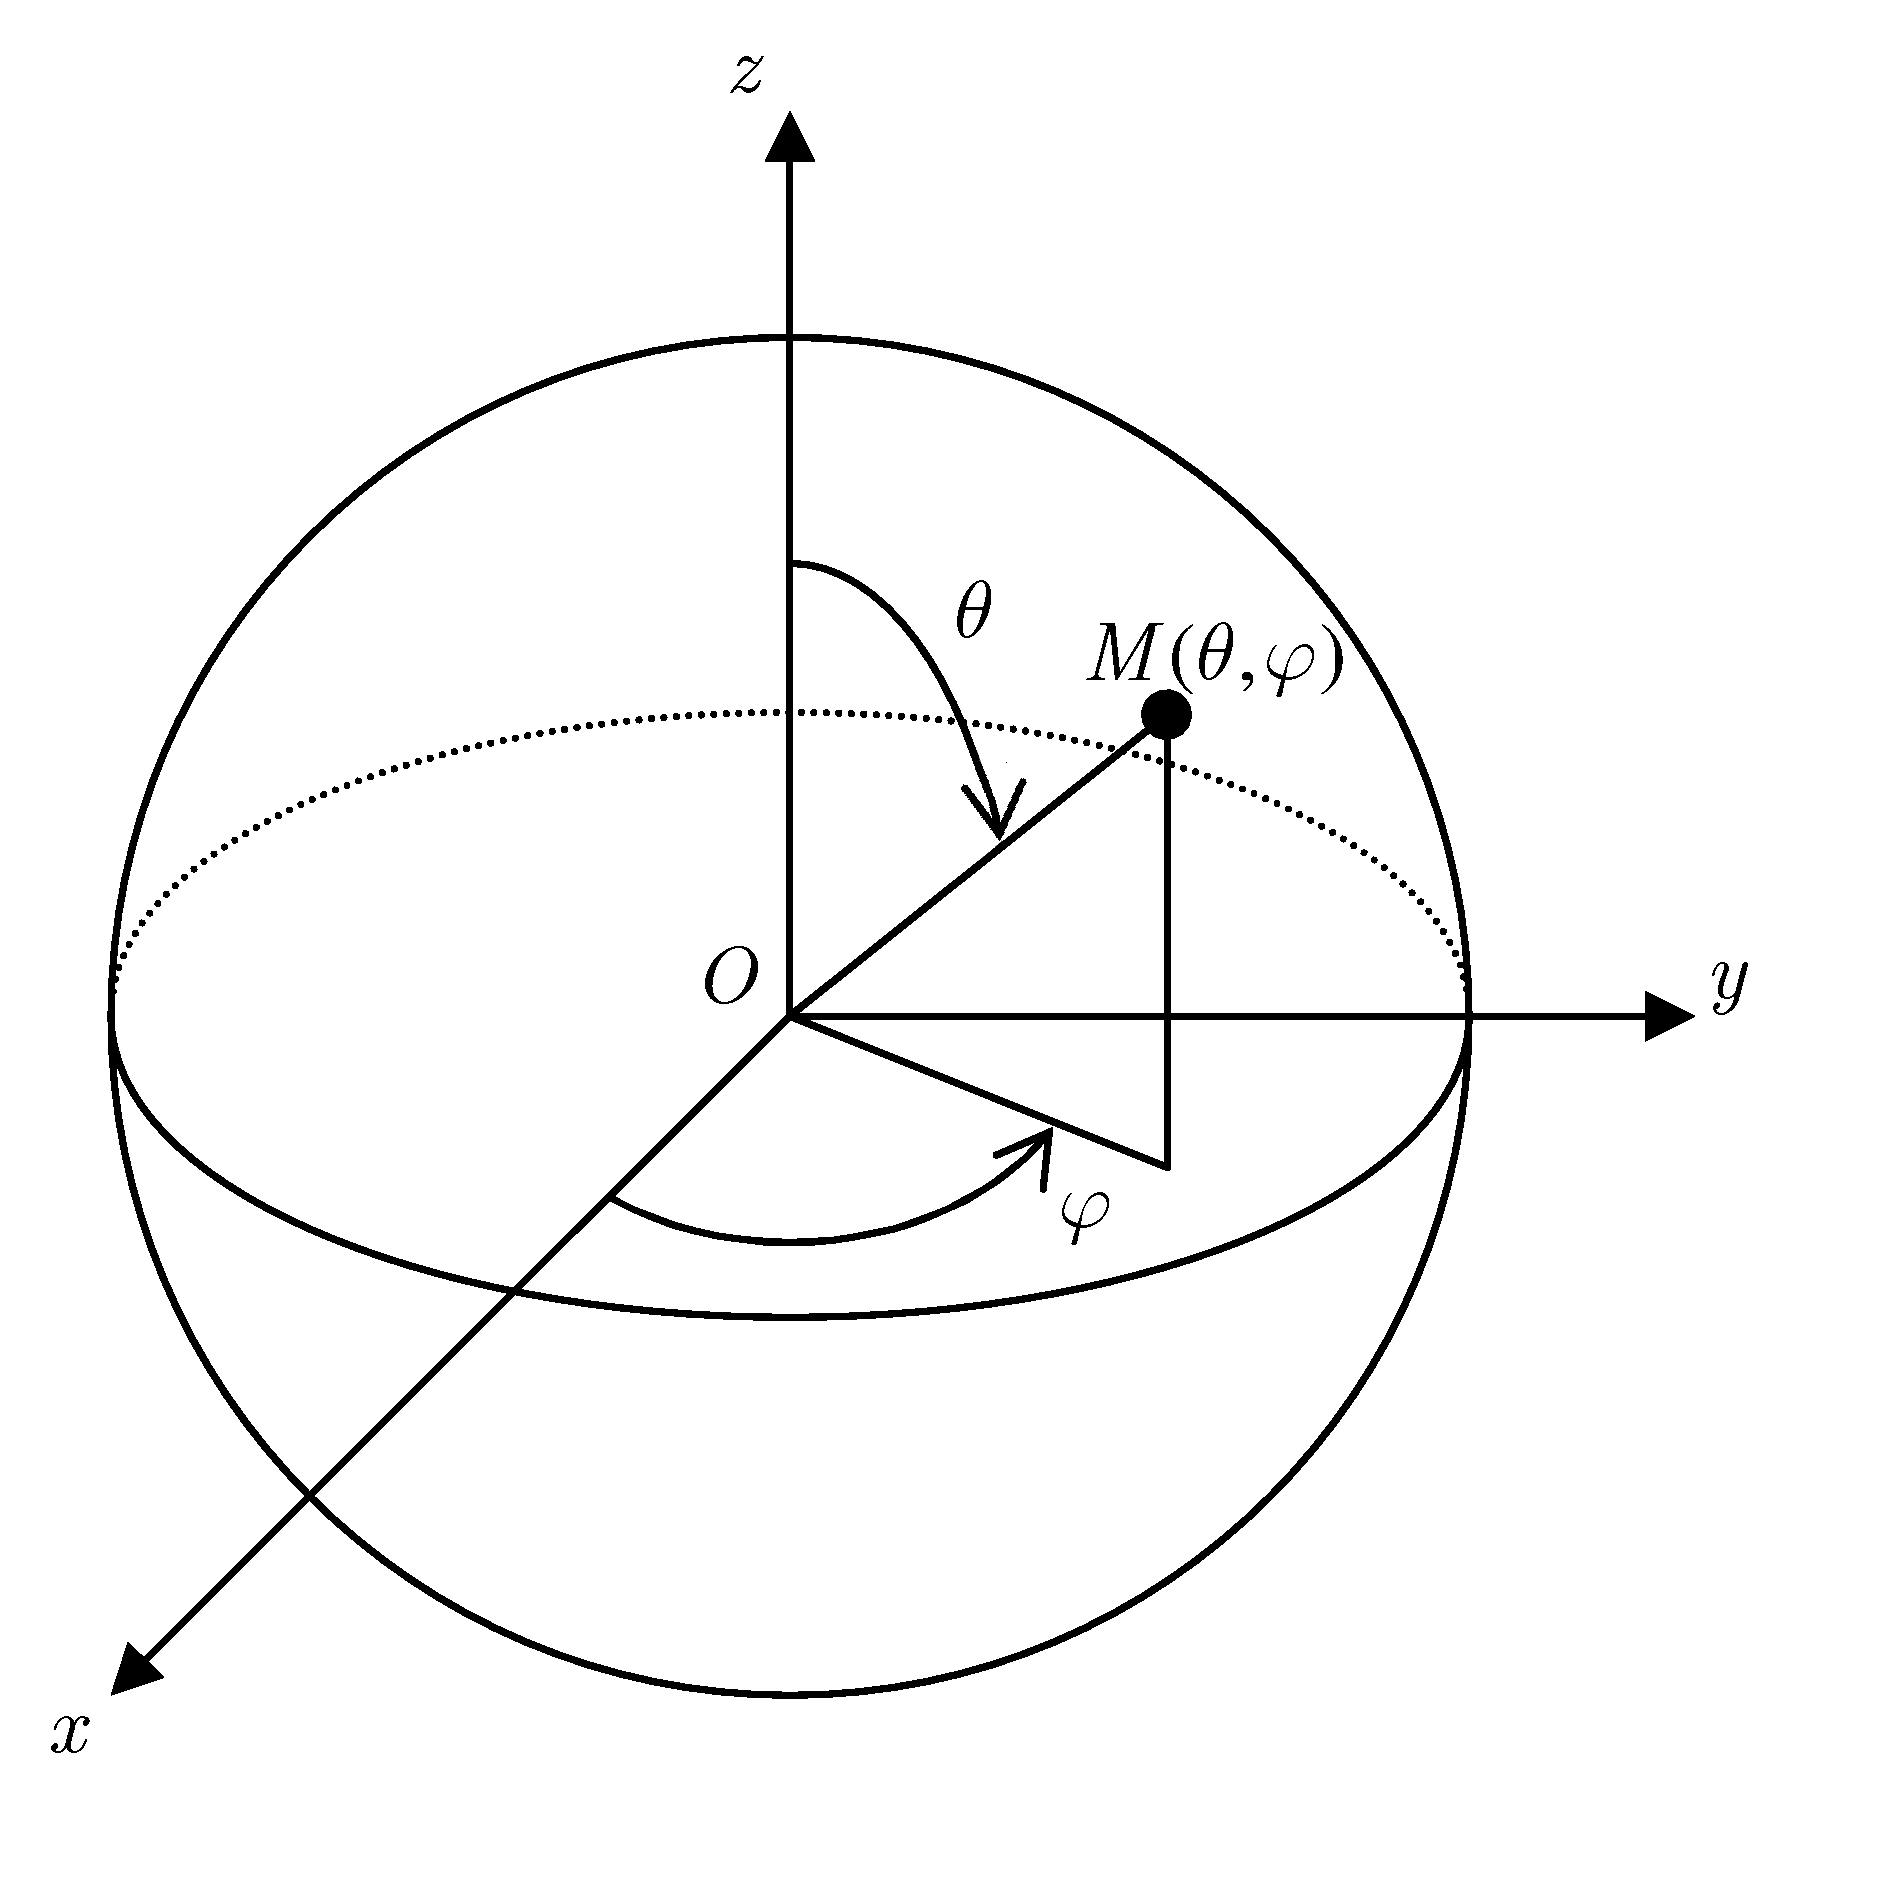
\includegraphics{repere.png}}
]{
\newline
On a donc les relations de passage suivantes:\\
\newline
$\left\{
\ba{rcl}
x&=&r\cos\pphi\ \cos\theta\\
y&=&r\cos\pphi\ \sin\theta\\
z&=&r\sin\pphi
\ea
\right.$, $\theta\in[0,\pi],\pphi\in[0,2\pi]$
\newline
\newline
et
\newline
\newline
$\left\{
\ba{rcl}
\h{r}&=&\sin\theta\ (\cos\pphi\ \h{x}+\sin\pphi\ \h{y})+\cos\theta\ \h{z}\\
\h{\theta}&=&\cos\theta\ (\cos\pphi\ \h{x}+\sin\pphi\ \h{y})-\sin\theta\ \h{z}\\
\h{\pphi}&=&-\sin\pphi\ \h{x}+\cos\pphi\ \h{y}
\ea
\right.$
\newline
\newline
\newline
Les variables d'espace $x,y,z$ seront respectivement conjuguées
aux variables spectrales $k_x,k_y,k_z$ par transformée de Fourier \eqref{tf}.
}
\emc
\end{figure}


Les variables d'intérêt étant ici les variables d'espace (et non pas le temps), nous considérerons implicitement
que toutes les relations sont valables à tout instant $t$ fixé.
Nous travaillerons en régime harmonique (convention $\e^{-i\omega t}$).
Ainsi, les constantes seront considérées en amplitudes complexes,
avec par exemple, $E_0=E\e^{-i\omega t}$ pour tout $E_0$ constant par rapport aux variables d'espace.
Dans la suite du rapport, une variable sera dite constante lorsque qu'elle ne dépendra pas des variables d'espace.


\subsection{Modélisation, définitions}


Le milieu considéré, l'air, sera assimilé au vide dans tout le rapport.


\begin{defi}[Onde plane étudiée]\label{OPPH}
On étudie une onde plane progressive harmonique polarisée rectilignement (OPPHPR),
représenté en \ref{decomposition} par la projection $\v{E}$ sur le plan $(xOy)$ de sa composante électrique.
\footnote{En effet, toute onde électromagnétique est une superposition d'OPPHPR, comme expliqué dans \cite{OptiqueEM}.\\
De plus, à partir de cette projection, il est possible retrouver la composante du champ
selon $\h{z}$, et ainsi reconstituer le champ global.}

On peut donc écrire $\v{E}$ sous la forme
$\v{E}=\v{E}_0\exp(i\v{k}_i\cdot\v{r})$, où:

\begin{itemize}
 \item $\v{E}_0=E_0\h{u}$ désigne un champ électrique constant
 \item $\v{r}=x\h{x}+y\h{y}+z\h{z}=r\h{r}$ désigne le vecteur position du point de l'espace considéré
 \item $\v{k}_i=k_0\h{k}_i$ désigne le vecteur d'onde initial,
 $k_0$ étant donc le nombre d'onde ($\h{k}_i\perp\h{u}$)
 \item $\lambda_0=\ff[2\pi]{k_0}$ désigne la longueur d'onde considérée.
\end{itemize}

Notons $k_{ix}=\v{k}_i\cdot\h{x}$, $k_{iy}=\v{k}_i\cdot\h{y}$, et $k_{iz}=\v{k}_i\cdot\h{z}$; alors on a:

\be
\v{E}=\v{E}_0\exp\lb i\v{k}_i\cdot(x\h{x}+y\h{y}+z\h{z})\rb = \v{E}_0\exp\lb i(xk_{ix}+yk_{iy}+zk_{iz})\rb
\label{0}
\tag{0}
\ee

\end{defi}

\newpage


\begin{defi}[Frame de Gabor, pas de translations, limites]\label{frame}

Le frame de Gabor associé à la fenêtre $w(x)$ considérée est défini par l'ensemble des fonctions
modulées et translatées $(w_{mn})_{m,n\in\Z}$ tel que: 

\be
\forall m,n\in\Z, w_{mn}(x)=w(x-m\b{x})\e^{inx\b{k}_x}
\label{wmn}
\ee

où $\b{x}$ et $\b{k}_x$ sont respectivement les pas de translations spatiale et spectrale.

On notera $A$ et $B$ les limites respectivement inférieure et supérieure du frame.

\end{defi}

$w_{mn}(x)$, $\b{x}$, et $\b{k}_x$ seront respectivement notés
$wmn(m,n,x)$, $xb$, et $kxb$ dans le script associé au rapport.


\begin{defi}[Frame de Gabor dans le domaine spectral]

Le frame de Gabor associé à la fenêtre $\t{w}(k_x)$ transformée est défini par l'ensemble
des fonctions modulées et translatées $(\t{w}_{nm})_{n,m\in\Z}$ tel que: 

\be
\forall m,n\in\Z, \t{w}_{nm}(k_x)=w(k_x-n\b{k}_x)\e^{-im\b{x}k_x}
\label{wtnm}
\ee

Ce frame est de limites $2\pi A$ et $2\pi B$.

\end{defi}

$w_{nm}(k_x)$ sera notée
$wtnm(n,m,kx)$ dans le script associé au rapport.


\begin{Rem}[Indices de translations]

Les indices $m$ et $n$ sont \emph{respectivement} les indices de translations spatiale et spectrale,
et ce, quelque soit le domaine dans lequel on considère notre fenêtre.
L'inversion de l'ordre de $m$ et $n$ dans la notation de $(\t{w}_{nm})$ est donc cohérente avec le fait
qu'une translation dans le domaine spatial correspond à une modulation dans le domaine spectrale,
et réciproquement.

Nous tâcherons de respecter ces notations (translation sur la première variable,
modulation sur la deuxième), notamment dans le programme associé à ce rapport.

\end{Rem}


Comme détaillé en \ref{AB}, $A$ et $B$ dépendent du coefficient d'échantillonnage défini juste après.


\begin{defi}[Coefficient d'échantillonnage]

Le coefficient d'échantillonnage associé au frame de Gabor précédent est:

\be
\nu_x=\f[\b{x}\b{k}_x]{2\pi}
\label{nux}
\ee

D'après le théorème de Balian-Low \cite{Balian}, les fenêtres considérées étant gaussiennes,
il faut que $\nu_x<1$ pour avoir effectivement des frames avec une bonne localisation
dans les domaines spatial et spectral.

\end{defi}

$\nu_x$, $A$ et $B$ seront donc respectivement notés
$nux$, $A[nux]$, et $B[nux]$ dans le script associé au rapport.


\begin{defi}[Largeur de fenêtre gaussienne]

Notons $w(x)=\r{\ff[\r{2}]{L_x}}\e^{-\pi\lc\ff[x]{L_x}\rc^2}$
toute fenêtre gaussienne de la variable $x$.
Alors $L_x$ désigne la largeur de fenêtre gaussienne.

Dans toute la suite du rapport, on se place dans \emph{l'hypothèse du frame équilibré}, on pose donc:
\be
\b{x}=\r{\nu_x}L_x
\tag{3.1}
\label{Lx}
\ee

\end{defi}


\begin{defi}[Largeur spectrale]

Notons $\t{w}(k_x)=\r{\r{2}L_x}\e^{-\pi\lc\ff[k_x]{\Omega_x}\rc^2}$
la transformée de Fourier de $w$.
Alors $\Omega_x$ désigne la largeur spectrale. On a: $\Omega_x=\f[2\pi]{L_x}$.
L'hypothèse du frame équilibré donne donc la relation:

\be
\b{k}_x=\r{\nu_x}\Omega_x
\tag{3.2}
\label{Ox}
\ee

\end{defi}


\begin{defi}[Frame dual dans le domaine spatial]

Le frame dual associé au frame $(w_{mn})$ est défini par l'ensemble
des fonctions $(\h{w_{mn}})_{n,m\in\Z}$ tel que: 

 \be
 \forall m,n\in\Z, \h{w_{mn}}(x)=\h{w}_{mn}(x),\ \h{w}=S^{-1}(w)
 \label{wdmn}
 \ee

$S$ étant \og l'opérateur de frame \fg\ ($S$ et $S^{-1}$ sont linéaires).
Ce frame est de limites $B^{-1}$ et $A^{-1}$.

\end{defi}


\begin{defi}[Frame dual dans le domaine spectral]

Le frame dual associé au frame $(\t{w}_{nm})$ est défini par l'ensemble
des fonctions $(\h{\t{w}_{nm}})_{n,m\in\Z}$ tel que: 

 \be
 \forall m,n\in\Z, \h{\t{w}_{nm}}(k_x)=\h{\t{w}}_{nm}(k_x)
 \label{wtdnm}
 \ee

Ce frame est de limites $(2\pi B)^{-1}$ et $(2\pi A)^{-1}$.

\end{defi}

$L_x$, $\t{w}(k_x)$, $\Omega_x$, $\h{w}(x)$... seront respectivement notés
$Lx$, $wd(kx)$, $Ox$, $wd(x)$... dans le script.


%Remarque: $S$ et $\F$ ne commutent pas: voir par exemple la formule \eqref{duals}.


\begin{Rem}[Extension en dimension 2 et 3 par séparabilité]
 
 Dans la suite du rapport et notamment dans le \ref{decomposition},
 les formules utilisées seront des extensions en deux dimensions des formules issues de la théorie des frames,
 mais qui ne sont pas toutes reportées ici afin de ne pas alourdir le propos. La clé de cette extension est
 \emph{la séparabilité}; se référer à \cite{TheseLugara} pour plus de détails.

 \end{Rem}
 

\newpage